%*****************************************
\chapter{Evaluation}\label{ch:evaluation}
%*****************************************

Test data was generated on a laptop running Linux Mint 10.0 using a 1.46 Ghz Intel Pentium dual core CPU with 1 GiB of RAM. A 10 Mbpbs broaband connection was used to connect to the internet, with measured download/upload rates of around 8 Mbps and 2 Mbps respectively.

For comparison, Firefox 4.0's minumum requirements include a single core 1.4 Ghz CPU with 512Mb of RAM \cite{firefox-req}. The average broadband speed in the UK is around 10 Mbps \cite{bband-stats}. 



\section{Conduit image performance}

The per-image channel capacity is a the function of the amount of information the implementation can store in a single image (equivalently - the symbol size) and the bit error probability. We model the compression/decompression process as a binary symmetric channel and calculate the channel capacity for arbitrarily small error probability, using the empirical bit error rate as an estimate for the bit error probability.

When used in conjunction with a forward error correction scheme we can also consider the actual per-image useful data rate and final decoder output error probability.


\subsection{Method}

The relevant library components are loaded into a test C++ application. A standalone conduit image instance is created and a random byte vector generated and encoded. The result is saved to disk as a JPEG at a given quality factor, reloaded and the data decoded. We log the Hamming distance between the input and output data. This process is repeated until the cumulative amount of data processed exceeds 1 GiB. The test was repeated for each of the three conduit image classes and also for quality factors 80-90.

\begin{table}[tbph]
  \begin{center}
        \begin{tabular}{l l l l l}
        \textbf{Method} &\textbf{Bits per} &\textbf{Test set size} & \textbf{Test set size} &\textbf{Possible unique} \\ 
            &\textbf{block} &\textbf{(images)} &\textbf{(blocks)} &\textbf{blocks} \\ [0.1ex] \hline \\ [-1.5ex]
        Scaled3	&192	&5,523	&44,736,300	& $6.28 \times 10^{57}$ \\
        Scaled4	&256	&4,142	&33,550,200	& $1.16 \times 10^{77}$ \\
        Haar	&24	&44,186	&357,906,600	& $1.68 \times 10^{7}$ \\
        \end{tabular}
        \caption{Tabulated details of the testing process. \textasciitilde 1 GiB of data was used for every test run.}
        \label{tab:img-test}
    \end{center}
\end{table}

Table \ref{tab:img-test} summerises the number of useful bits each method can store in a single 64 x 8 bit greyscale JPEG luminance block along with the effective sample size (number of images/blocks processed during the test) and population size (total number of possible unique blocks) we are sampling from. Due to the size of the samples the standard error is negligable, even before applying finite population correction where appropriate \footnote{In particular, for the Haar wavelet transform method the number of JPEG blocks encoded exceeds the number of unique datapoints that can be encoded in a single block.}. 


\subsection{Theoretical capacity}

\begin{figure}[tbph]
  \begin{center}
\begin{tikzpicture}
    \begin{axis}[grid=major,xlabel=JPEG Quality Factor,ylabel=BER (\%), xmin=80, xmax=90,
    height=9cm,width=11cm,legend style={legend pos=outer north east}]
    
    \addplot
        table[x=QF,y=Sc3] {gfx/error_rate.data};
    
    \addplot
        table[x=QF,y=Sc4] {gfx/error_rate.data};
        
    \addplot
        table[x=QF,y=Haar] {gfx/error_rate.data};
        
    \legend{Scaled3,Scaled4,Haar}
    
    \end{axis}
\end{tikzpicture}
    \caption{Bit error rate for varying quality factors.}
    \label{graph:ber}
  \end{center}
\end{figure}

Figure \ref{graph:ber} charts bit error rates for each implementation. As expected, rates generally decrease as the quality factor increases. All three methods show a marked improvement over the naive approaches detailed in section TODO.

\begin{figure}[tbph]
  \begin{center}
\begin{tikzpicture}
    \begin{axis}[grid=major,xlabel=JPEG Quality Factor,ylabel=Capacity (KiB/image), xmin=80, xmax=90,
    height=9cm,width=11cm,legend style={legend pos=outer north east}]
    
    \addplot
        table[x=QF,y=Sc3] {gfx/encoding_time.data};
    
    \addplot
        table[x=QF,y=Sc4] {gfx/encoding_time.data};
        
    \addplot
        table[x=QF,y=Haar] {gfx/encoding_time.data};
        
    \legend{Scaled3,Scaled4,Haar}
    
    \end{axis}
\end{tikzpicture}
    \caption{Per-image channel capacity (measured in KiB/image) for varying quality factors.}
    \label{graph:capacity}
  \end{center}
\end{figure}

We model each conduit image as a binary symmetric channel: we know the encoding/decoding process does not result in bit erasures; we make the assumption that the probability of error $p_e$ is independant and equal for each bit. Given the large sample sizes we can assume that the measured bit error rate is a reasonable estimate of the actual bit error probability.

The formula used to calculate the capacity is obtained by taking the typical capacity calculation for a binary symmetric channel and multiplying by the number of bits available per image $A$, to obtain:

\begin{equation}
    C = A \cdot (1 + H(p_e))
\end{equation}

Where $H(x)$ is the binary entropy function. This provides the capacity in units of information per symbol - in this case bits per image. Figure \ref{graph:capacity} compares the calculated capacity for each of the three conduit images implementations. At quality factor 85, which most closely matches the profile of the Facebook JPEG compression proccess, we see both scaling methods performing approximately the same with capacities of over 180 KiB per image.


\subsection{Reed Solomon error correction}

Given the bit error probability $p$ we can obtain the symbol error probability $p_s$:

\begin{equation}
    p_s = 1 - (1-p)^m
\end{equation}

where $m$ is the number of bits per symbol. In general, for a Reed Solomon code with symbol error probability $p_s$ the decoded symbol error probability $p_s'$ is given by:

\begin{equation}
    p_s' = \frac{1}{2^m -1} \sum^{2^m - 1}_{i = t+1} i {{2^m - 1}\choose{i}} {p_s}^i (1-{p_s})^{2^m - 1 - i}
\end{equation}

where $t$ is the maximum number symbol errors we can correct \cite{rsfec-decode}. Both the error correction classes in the Encrypted Facebook library are based on Reed Solomon codes. The (15,9) code can correct up to $t=3$ symbol errors and has a 4-bit symbol size. The (255,223) code can correct up to $t=16$ symbol errors and has a 8-bit symbol size.

Figure \ref{tab:fec} tabulates error probabilities for each FEC scheme used; again we use the
measured bit error rate as an estimate of the bit error probability. The decoded symbol error probability $p_s'$ we may consider as an upper bound for the decoded bit error probability. 

\begin{table}[tbph]
  \begin{center}
        \begin{tabular}{l l l l l l}
            
            \textbf{Method} & \textbf{FEC} & \textbf{$p$} & \textbf{$p_s$} & \textbf{$p_s'$} & \textbf{Capacity} \\  & &  &  &  & \textbf{(KiB)} \\[0.1ex] \hline \\ [-1.5ex]

            Haar & (15,9) & $4.20 \times 10^{-3}$ & $1.67 \times 10^{-2}$ & $2.47 \times 10^{-5}$ & 14.2 \\
            Haar &  (255,223) & $4.20 \times 10^{-3}$ & $3.31 \times 10^{-2}$ & $3.73 \times 10^{-4}$ & 20.8 \\
            Scaled3 & (15,9) & $8.30 \times 10^{-4}$ & $3.32 \times 10^{-3}$ & $4.28 \times 10^{-8}
$ & 113.9 \\
            \rowcolor{green!50!white} Scaled3 & (255,223) & $8.30 \times 10^{-4}$ & $6.62 \times 10^{-3}$ & $1.81 \times 10^{-13}
$ & 166.0 \\
            Scaled4 & (15,9) & $4.49 \times 10^{-2}$ & $1.68 \times 10^{-1}$ & $7.14 \times 10^{-1}$ & 151.9 \\
            Scaled4 & (255,223) & $4.49 \times 10^{-2}$ & $3.08 \times 10^{-1}$ & $3.08
 \times 10^{-1}$ & 221.4 \\
            
        \end{tabular}
        \caption{Bit error probability, symbol error probability and output symbol error probability for each possible combination. Quality factor is 85.}
        \label{tab:fec}
    \end{center}
\end{table}


\subsection{Conclusion}

The Haar wavelet class has too low a capacity (at any quality factor) to be used in practise, though the low bit error rates logged support the claim (see XXX) that such an encoding is reasonably immune to JPEG compression. In addition, there is anecdotal evidence that suggests that $p_s'$ in Figure \ref{tab:fec} is not a particularly tight bound on the actual output bit error probability - during the testing in section XXX several megabytes of data were encoded, uploaded and retrieved successfuly. 

The 4-bit-per-pixel 'Scaled4' class produced a bit error rate too high to be corrected with the Reed Solomon codes used here. Implementing a forward error scheme with a lower code rate would make this feasible - in particular if the JPEG quality factor were higher than 85 this method could potentially offer the highest capacity of the three classes tested.

The 3-bit-per-pixel 'Scaled3' class along with Reed Solomon (255,223) codes (highlighted in green) demonstrates a feasible combination (see XXX). Under this scheme we would expect less than one bit error in a terrabyte of encoded data. For comparison, this approaches hard disk drive read error rates \footnote{Stated by at least one hard drive vendor to be 1 uncorrectable read error in $10^{14}$ bits, or 10 terabytes \cite{hdd-errors}.}. For these reasons the remainder of the evaluation will focus on this implementation.



\section{Submission and retrieval times}

We consider the encode/decode and upload/download times for a single object, encoded using the 'Scaled3' class. Effects of asynchronous retrieval of multiple objects and caching of plaintext information locally are covered in section XXX.  


\subsection{Method}

Automated tests were ran programmatically from the extension, with each submission and retrieval round being allowed to complete entirely before beginning the next. All encryption was performed with a simulated group size of 405 as detailed in section XXX. Test images were duplicate copies of a (approximately) 50 KiB JPEG image (see section XXX). Test messages were randomly generated strings of mixed-case letter and numeral characters, 10,000 characters in length - the limit for private messages.

For textual content, 1000 messages were generated. The note submission function was then called with each message using a 60 second delay in between each run - leaving enough time for one submission and retrieval round to complete before beginning another. The tags required to retrieve these notes are saved and the time spent in each submission phase profiled. When the HTTP request for sumbmission completes, retrieval is triggered and the download and decoding time logged. The same test was repeated using a set of 1000 images.

All retrieved objects were compared with the originals to ensure error free transfer had occured. A modified version of the Chromebug Firefox extension was used to record all results.


\subsection{Results}

For text messages times were dominated by the HTTP transfer; encoding and decoding times were negligable. For images the encoding and decoding times were more significant, in particular when retrieveing where more time was spent decoding the image than downloading.

\begin{figure}[tbph]
    \begin{center}
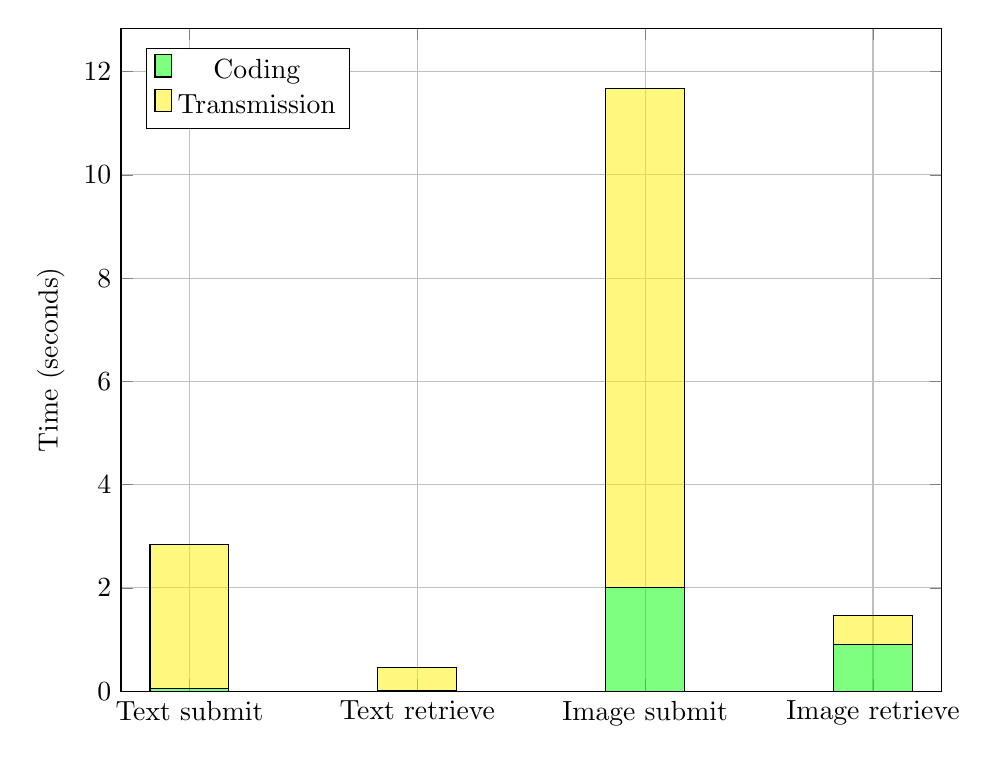
\begin{tikzpicture}
\begin{axis}[grid=major,ybar stacked, 
    symbolic x coords={Text submit,Text retrieve, Image submit, Image retrieve},
    xtick=data,ylabel=Time (seconds), width=12cm, height=10cm,
    legend style={legend pos=north west, area legend},
    bar width=1cm, ymin=0]

    \addplot[fill=green, fill opacity=0.5] coordinates
    {(Text submit,0.0444) (Text retrieve,0.0172) (Image submit,2.0074) (Image retrieve,0.9044)};
    
    \addplot[fill=yellow, fill opacity=0.5] coordinates
    {(Text submit,2.8013) (Text retrieve,0.4446) (Image submit,9.6655) (Image retrieve,0.5662)};
    
    \legend{Coding,Transmission}

\end{axis}
\end{tikzpicture}
    \caption{Average timing results for a 10,000 chracter note and an (approximately) 50 KiB image.}
    \label{graph:txt-sync}
  \end{center}
\end{figure}



\section{Effect of cache on loading times}

We evaluate the effect of caching plaintext items that have already been retreived when loading an entire page. Here we also condider DOM tree navigation/insertion operations and asynchronous object retrieval. Pages containing multiple items of encrypted content were loaded, triggering asynchronous retrieval and deocoding.


\subsection{Method}

Sample newsfeeds were generated with 15 encrypted status update entries, as this is the number of newsfeed entries Facebook first loads \footnote{More are loaded dynamically when the user scrolls to the bottom of the page.}. Status update messages were random ASCII text 420 characters in length, the maximum permitted. The pages were loaded repeatedly 400 times, ensuring that both the browser cache and extension cache were cleaned after each load.

The entire process was then repeated for a newsfeed containing 15 image objects, once again random images of size 50 KiB, instead of status messages. In addition, a second set of test were performed without cleaning the extension cache (which was preloaded with the page's content).

The start time of each test was logged, along with the 15 subsequent load times of the encyrpted objects. 


\subsection{Results}

The effect of plaintext caching on the overall page loading times can be seen in figure \ref{graph:hist}. Caching provided a factor 2 speed increase for text and a factor 4 increase for images.

\begin{figure}[tbph]
    \begin{center}
\begin{tikzpicture}
\begin{axis}[xlabel=Time (seconds), ylabel=Frequency,
grid=major,const plot, ymin=0, enlargelimits=false,
width=12cm, height=5cm, legend style={area legend}]

    \addplot[fill=blue, fill opacity=0.5] table[x=t,y=Text] {gfx/async_text_hist.data};
    
    \addplot[fill=red, fill opacity=0.5] table[x=t,y=Text_c] {gfx/async_text_hist.data};
    
    \addplot+[sharp plot,blue, mark=no marker] coordinates
        {(6.403,0) (6.403,56)};
        
    \addplot+[sharp plot,red, mark=no marker] coordinates
        {(3.463,0) (3.463,56)};
    
    \legend{Cache off,Cache on}
\end{axis}
\end{tikzpicture}

\begin{tikzpicture}
\begin{axis}[xlabel=Time (seconds), ylabel=Frequency,
grid=major,const plot, ymin=0, enlargelimits=false,
width=12cm, height=5cm, legend style={area legend}]
    
    \addplot[fill=blue, fill opacity=0.5] table[x=t,y=Images] {gfx/async_image_hist.data};
    
    \addplot[fill=red, fill opacity=0.5] table[x=t,y=Images_c] {gfx/async_image_hist.data};
    
    \addplot+[sharp plot,blue, mark=no marker] coordinates
        {(19.169,0) (19.169,130)};

    \addplot+[sharp plot,red, mark=no marker] coordinates
        {(4.067,0) (4.067,130)};
    
    \legend{Cache off,Cache on}
    
\end{axis}
\end{tikzpicture}
    \caption{Histogram of 400 page loading times for newsfeeds containing 15 encrypted messages (top) and 15 encrypted images (bottom).}
    \label{graph:hist}
  \end{center}
\end{figure}

If we consider the time that the user is kept waiting then the results are even more dramatic. Since there is a significant difference between the waiting time for the first loaded object and the subsequent waiting times for the remainder, we consider them seperately.

From figure \ref{graph:time-first} we again see a modest improvement in loading times. However, looking at figures \ref{graph:txt-rest} and \ref{graph:img-rest} we see that the time spent waiting in between loads has now dramatically decreased - to around 6 ms or less for either text or images. This is as we would expect since the only work required from the application is creating source references to images on disk and inserting elements into the DOM tree.

\begin{figure}[tbph]
    \begin{center}
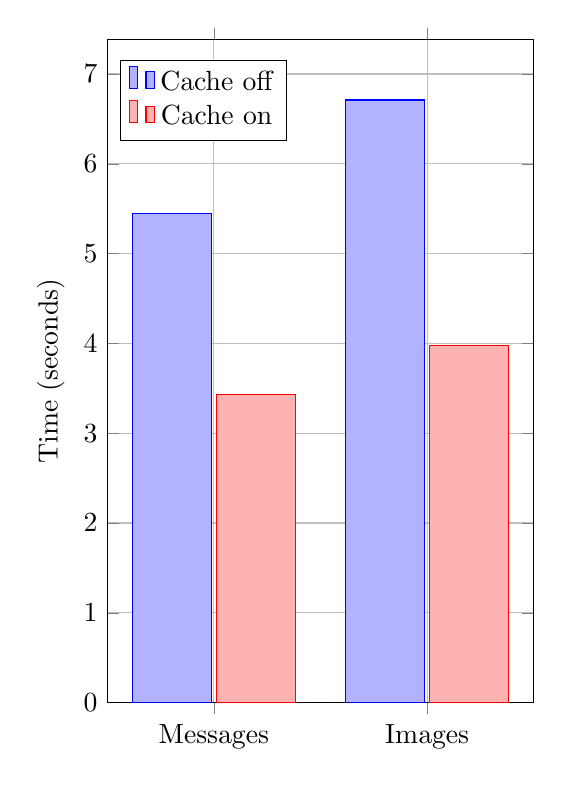
\begin{tikzpicture}
\begin{axis}[grid=major,ybar, 
    symbolic x coords={Messages,Images},
    xtick=data,ylabel=Time (seconds), width=7cm, height=10cm,
    legend style={legend pos=north west, area legend},
    bar width=1cm,enlarge x limits=0.5,ymin=0]
        \addplot coordinates { (Messages,5.4457) (Images,6.7105) };
        \addplot coordinates { (Messages,3.4306) (Images,3.9765) };
        \legend{Cache off, Cache on}
\end{axis}
\end{tikzpicture}
    \caption{Average time before first encrypted item loads.}
    \label{graph:time-first}
  \end{center}
\end{figure}

\begin{figure}
    \begin{center}
        \begin{tikzpicture}
        \begin{axis}[grid=major,ycomb,
        ylabel=Time (ms), 
        width=12cm, height=5cm,
        bar width=0.3cm, ymin=0, xmin=2, xmax=15, enlarge x limits=0.04]
            \addplot[blue] table[x=Item,y=Text] {gfx/async.data};
        \end{axis}
        \end{tikzpicture}
        \begin{tikzpicture}
        \begin{axis}[grid=major,ycomb,
        ylabel=Time (ms), xlabel=Message,
        width=12cm, height=5cm,
        bar width=0.3cm, ymin=0, xmin=2, xmax=15, enlarge x limits=0.04]
            \addplot[red] table[x=Item,y=Text_c] {gfx/async.data};
        \end{axis}
        \end{tikzpicture}
    \caption{Average time interval between successive message loads, with caching turned off and on (top and bottom respectively).}
    \label{graph:txt-rest}
    \end{center}
\end{figure}
\begin{figure}[tbph]
\begin{center}
    
\begin{tikzpicture}
\begin{axis}[grid=major,ycomb,
ylabel=Time (ms), 
width=12cm, height=5cm,
bar width=0.3cm, ymin=0, xmin=2, xmax=15, enlarge x limits=0.04]
    \addplot[blue] table[x=Item,y=Image] {gfx/async.data};
\end{axis}
\end{tikzpicture}

\begin{tikzpicture}
\begin{axis}[grid=major,ycomb,
ylabel=Time (ms),xlabel=Image,
width=12cm, height=5cm,
bar width=0.3cm, ymin=0, xmin=2, xmax=15, enlarge x limits=0.04]
    \addplot[red,] table[x=Item,y=Image_c] {gfx/async.data};
\end{axis}
\end{tikzpicture}

\caption{Average time interval between successive image loads, with caching turned off and on (top and bottom respectively).}
\label{graph:img-rest}
\end{center}
\end{figure}

\section{Useability inspection}

A full user study was considered too time consuming to perform; instead we use a cognitive walkthrough (as described by Wharton et al \cite{cogwalk}) to evaluate the success of the user interface. During development many passes of the walkthrough were perfomed and alterations made, until a credible success story could be constructed for each task. This section consists of a selection of some of the final success stories and a defense of their validity.

We only consider one class of user - a typical Facebook user who is therefore familiar with the Facebook user interface. It is therefore assumed that actions such as "navigate to a given friend's profile" can be performed without additional aid. It is also assumed that the user will follow their usual actions when trying to perform an encrypted operation - when trying to upload an encrypted image they will, for example, simply follow the normal procedure for uploading an image rather than searching for some hidden option. Finally, we make the assumption that the extension has been installed and enabled and that the toolbar has not been hidden.


\subsection{Creating a cryptographic identity}
A user who is not logged in but who knows the extension is installed, wishes to make use of some of the extensions functionality and his actions result in the creation of a (prerequisite) cryptographic identity.

\begin{description}

    \item[Action Sequence] \hfill
    
    \begin{enumerate}
        \item Log in to Facebook.
        \item Click on the {\tt [Create Identity]} button.
        \item Enter a password according to the restrictions.
        \item Re-enter password.
    \end{enumerate}
    
    \item[Defense of Credibility] \hfill
        \begin{itemize}
            
            \item The user knows to click the {\tt [Create Identity]} button. We know the user wants to use the extension in some way and is aware that the plugin is installed - it is reasonable to assume that he will look at the toolbar. All other buttons are greyed out, and the process of creating some form of identity/account/profile before using a service is familiar to anyone who has used Facebook, or any other site which requires membership.
            
            \item If the user isn't logged in to Facebook, he knows he must first do so since he will be informed of this on clicking {\tt [Create Identity]}. User will know how to log in to Facebook.
            
            \item User will know how to cancel process as it is clearly marked.
            
            \item Quiting/crashing the browser or cancelling will result in a return to the initial state.
            
            \item User will either enter a valid password or be prompted by the restrictions on entering an invalid one, in which case he will then know how to enter a valid password and do so.
            
            \item User will know if he incorrectly re-enters password via an alert.
            
            \item User knows things are OK because an alert informs him the process was succesful.
            
        \end{itemize}
\end{description}

\subsection{Logging in to a cryptographic identity}
A user who is not logged in but has created an identity, wishes to make use of some of the extensions functionality and logs in.

\begin{description}

    \item[Action Sequence] \hfill
    
    \begin{enumerate}
        \item Log in to Facebook.
        \item Click on the {\tt [Start Encrypted Facebook]} button.
        \item Enter user password.
    \end{enumerate}
    
    \item[Defense of Credibility] \hfill
        \begin{itemize}
            
            \item User knows to click {\tt [Start Encrypted Facebook]} . We know the user wants to use the extension in some way and is aware that the plugin is installed - it is reasonable to assume that he will look at the toolbar. All other buttons are greyed out apart from {\tt [Create Identity]} which he has used before. If he does mistakenly click {\tt [Create Identity]} he will be informed that he already has an identity and that attempting to overwrite it will result in irrevocable data loss.
            
            \item If the user isn't logged in to Facebook he knows he must first do so since he will be informed of this on clicking {\tt [Start Encrypted Facebook]}. User will know how to log in to Facebook.
            
            \item User will know his password and be able to enter it. In the case that the user doesn't know his password he will know he must create a new one and do so as described in section XXX.
            
        \end{itemize}
\end{description}

\subsection{Adding public keys}
A user with no public keys wishes to submit encrypted content. His actions lead to him obtaining one of his intended recipient's public key.

\begin{description}

    \item[Action Sequence] \hfill
    \begin{enumerate}
        \item Navigate to a friends profile.
        \item Click the {\tt [Add Public Key]} button.
    \end{enumerate}
    
    \item[Defense of Credibility] \hfill
    \begin{itemize}
        \item Assume that a user wishing to perform some encrypted operation knows what process to follow, as demonstrated in sections XXX and XXX. Attempting this process with no public keys will result in a prompt informing the user that they must navigate to a friends profile and click the {\tt [Add Public Key]} button in order to use them as a recipient.
    
        \item Facebook user will be familiar with the process of finding a friends profile and clicking on a button therein.
        
        \item User will know where the {\tt [Add Public Key]} button is since it is clearly labelled and positioned at the top of the page next to several normal Facebook buttons.
        
    \end{itemize}
    
\end{description}

\subsection{Using the recipient selector control}
A user presented with the recipient selector control wishes to use it to select a large subset of his friends for broadcast encryption, and does so. The user has 406 friends available to select and wants to choose 405 of them.

\begin{description}

    \item[Action Sequence] \hfill
    \begin{enumerate}
        \item Click the {\tt [Select all]} check button
        \item Deselect the friend who is to be excluded.
        \item Click the {\tt [Submit]} button in the popup window.
    \end{enumerate}
    
    \item[Defense of Credibility] \hfill
        \begin{itemize}
            
            \item User knows that the friend selector is used to select recipients as this is stated clearly abover the control.
            
            \item Users know generally how to select recipients by clicking on them one-by-one and also that they can deselect by clicking an already selected item, since this process of selecting recipients is familiar to them from general Facebook use and the UI control itself is based on Facebook's own. 
            
            \item User knows to click {\tt [Select all]}. The button is visible and clearly labelled; common sense would dictate that selecting all then deselecting one item would be quicker than selecting all 405 items individually.
            
            \item User knows things are OK. After clicking {\tt [Select all]} all items will switch to looking selected in a manner consistent with other controls used by Facebook.
            
            \item User knows how to deselect a friend. Again based on the familiarity with the control from Facebook we assume they are capable of scrolling through the alphabetical list to find their the friend in question.
            
            \item User knows to click {\tt [Submit]}. No button other than cancel is visible on the control, the button is clearly labelled and its appearance and position is based on Facebook's own controls.
            
            \item User knows things are OK as the popup responds to their click by disappearing, identical to the behaviour of a Facebook control.
        
        \end{itemize}
    
\end{description}


\subsection{Uploading an encrypted image}
A user wishing to send an encrypted image to 405 friends who also have the extension, does so.

\begin{description}

    \item[Action Sequence] \hfill
    \begin{enumerate}
        \item Add any public keys required.
        \item Navigate to the image upload page for the required album.
        \item Select the image to encrypted.
        \item Check the {\tt [Encrypt]} check box.
        \item Click the {\tt [Submit]} button.
        \item Use the friend selector to select recipients and submit.
    \end{enumerate}
    
    \item[Defense of Credibility] \hfill
        \begin{itemize}
            
            \item The user knows he must add punlic keys of recipients beforehand and how to do so. If the user has no public keys section XXX demonstrates that he will be able to add one of his intended recipients. Since the process is reasonably simple - simply navigate to their page and click a clearly marked button, we assume that any user who has performed it once can do so again if they wish, without further instruction. The link between adding public keys and being able to choose those friends as recipients should be fairly obvious; when the first key is added and encryption attempted again that same friend will appear as the only possible recipient.
            
            \item Facebook user will be familiar with the process of uploading an image. We assume a user trying to upload an encrypted image will be likely to try the method they are already familiar with.
            
            \item User knows things are OK since he sees the encryption check box option on arriving at the upload page. Check box leaves little room for confusion over whether an upload will or won't be encrypted.
            
            \item User knows to select an image to upload since the process is identical to uploading plaintext images.
            
            \item User knows to select {\tt [Encrypt]} check box since uploading an encrypted image is the original task.
            
            \item User knows things are OK since the recipient selector pops up.
            
            \item User knows how to use the recipient selector (see section XXX).
            
            \item User knows things are OK as Facebook handles the upload process from here as per normal, notifying user when the upload is complete.
            
        \end{itemize}
    
\end{description}


\subsection{Posting a comment}
A user has navigated to his newsfeed. He wishes to write an encrypted reply to a plaintext comment on a newsfeed post of an encrypted photo. It is assumed he already possesses the public keys required and can decrypt the photo in question.

\begin{description}

    \item[Action Sequence] \hfill
    \begin{enumerate}
        \item Select the comment box below the plaintext reply.
        \item Type comment in plaintext.
        \item Click the {\tt [Encrypt \& Submit]} button.
        \item Use the friend selector to select recipients and submit.
        \item Refresh the page to review comment.
    \end{enumerate}
    
    \item[Defense of Credibility] \hfill
        \begin{itemize}
            
            \item User knows to select the comment box. This is required for submitting a plaintext comment, we assume the user will try the method they are used to.
            
            \item User knows things are OK as the {\tt [Encrypt \& Submit]} appears once the textbox has focus.
            
            \item User knows to type in the comment - this is identical to submitting a plaintext comment.
            
            \item User knows to click {\tt [Encrypt \& Submit]}. The user is familiar with clicking a similiar submit button during plaintext entry. The button is positioned beside the {\tt [Submit]} for plaintext entry, is styled like the {\tt [Submit]} button and is clearly labelled. Submitting an encrypted comment is part of the original task.
            
            \item User knows how to use the recipient selector (see section XXX).
            
            \item User knows things are OK as Facebook handles the submission process from here as per normal. A loading icon appears breifly, then the comment itself appears.
            
            \item User knows that their submission was encrypted as this fact is stated as part of the comment encoding.
            
            \item User knows they must refresh the page to view their own comment. Even if this is their first encrypted submission, Facebook users will be familiar with the process of refreshing a page when something is not working or to view an update. If the user does not make the connection right away, when returning to the page and seeing the item decrypted automatically they should realise that encrypted text submissions are decrypted as a page first loads.
        
        \end{itemize}
\end{description}


